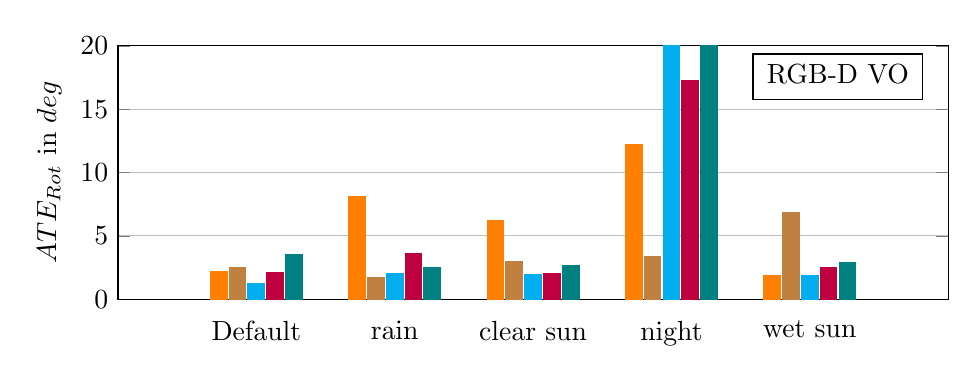
\begin{tikzpicture}
    \begin{axis}[
        width  = \textwidth,
        height = 4.8cm,
        ymax = 20,
        major x tick style = transparent,
        ybar=2*\pgflinewidth,
        bar width=6pt,
        ymajorgrids = true,
        ylabel = {$ATE_{Rot}$ in $deg$},
        % xlabel = {1 Default, 2 hard rain, 3 clear sunset, 4 clear night ,5 wet sunset},
        symbolic x coords={Default, rain, clear sun, night ,wet sun},
        xtick = data,
        scaled y ticks = false,
        enlarge x limits=0.25,
        ymin=0,
        legend pos=north east
    ]
    \addlegendimage{empty legend}
    \addlegendentry{RGB-D VO}
    \addplot[style={orange,fill=orange,mark=none}]
        coordinates {(Default, 2.21) (rain, 8.09) (clear sun, 6.195) (night ,12.18) (wet sun, 1.875)};
    
    \addplot[style={brown,fill=brown,mark=none}]
        coordinates {(Default,2.52) (rain, 1.73) (clear sun, 3.00) (night , 3.372) (wet sun, 6.825)};
    
    \addplot[style={cyan,fill=cyan,mark=none}]
        coordinates {(Default, 1.22) (rain, 2.00) (clear sun, 1.941) (night , 48.216) (wet sun, 1.838)};
    
    \addplot[style={purple,fill=purple,mark=none}]
        coordinates {(Default, 2.14) (rain, 3.60) (clear sun, 2.061) (night , 17.293) (wet sun, 2.518)};
    
    \addplot[style={teal,fill=teal,mark=none}]
        coordinates {(Default, 3.53) (rain, 2.493) (clear sun, 2.645) (night , 51.956) (wet sun, 2.893)};
    \end{axis}
  \end{tikzpicture}